\chapter{Teori}\label{Teori}
Dette kapitel beskriver teorien der er brugt til at udforme løsningen. Vi har i løsning brug grafteori til opstillingen af noderne og vejene der der forbinder noderne, samt brugen af grafen i A* til at finde den optimale rute gennem grafen. Pseudokoden der er vist ved Dijkstra og A* er omskrevet til vores egen stil, for at koden for begge algoritmer er på samme stil. Her bruges \texttt{end} til at afslutte løkke og procedurer, og kommandoer en if-sætning indeholder vises med indrykning.
\newpage
\section{Grafteori}

Grafteori handler om at beskrive  modeller matematisk. Grafteori er væslig når man skal optimere et netværk, det kunne f.eks. være en graf som representere et vejnetværk, hvor man her vil kunne bruge grafteori til bla rutefinding.  

En graf beskriver et par af mægnder, man kunne tag udgangspunkt i grafen G = (V,E) hvor V og E er mægnder. I eksempet her er V en ikke-tom mængde af knuder, og E er mængden af kanter som forbinder knuderne i mægnden V. 

\vspace{5mm}

Vi tager udgangpunkt i grafen på figur \ref{weighted-directed-graph}.

\begin{figure}[H]
\begin{adjustbox}{width=0.5\textwidth,center=\textwidth}
\centering
\includegraphics[width=0.5\textwidth]{Pictures/Teoriafsnit/Figurfiler/weighted_directed_graph.PNG}
\end{adjustbox}
\caption{Orienteret vægtet graf}
\label{fig:weighted-directed-graph}
\end{figure}

\vspace{5mm}

Man kan forstille sig dette er et vejnetværk, hvor punkterne(knuderne) representere sving, og linjerne(kanterne) er veje som forbinder svingene, samt beskriver tallet mellem 2 sving(knuder) lægnden(vægten) af vejen(kanten). Herved kan grafen godt forstille et simpel vejnetværk.

\vspace{5mm}

Vi kan udfra grafen se at knuderne \verb!"A, B, C, D, E, F \in V"!. 

\vspace{5mm}

Samt at kanterne \verb!"{A,B} \rightarrow 4 , {A,F} \rightarrow 5 , 
						{B,D} \rightarrow 7 , {C,A} \rightarrow 3 , 
						{C,B} \rightarrow 4 , {D,C} \rightarrow 2 ,!
						\\
				  \verb!{D,E} \rightarrow 3 , {E,D} \rightarrow 3 , 
				  		{E,F} \rightarrow 2 , {F,C} \rightarrow 1 , 
				  		{F,E} \rightarrow 1 \in  E"!

\vspace{5mm}

Grafen her kan derfor skrives rent matematisk:

\vspace{5mm}

\verb!G = (V,E), V = {A,B,C,D,E,F},! 

\vspace{5mm}

			\verb!E = { {A,B} \rightarrow 4 , {A,F} \rightarrow 5 , 
						{B,D} \rightarrow 7 , {C,A} \rightarrow 3 , 
						{C,B} \rightarrow 4 , {D,C} \rightarrow 2 ,!
						\\
				  \verb!{D,E} \rightarrow 3 , {E,D} \rightarrow 3 , 
				  		{E,F} \rightarrow 2 , {F,C} \rightarrow 1 , 
				  		{F,E} \rightarrow 1 \in  E" }!

\vspace{5mm}

En anden måde at repræsentere grafen på er ved hjælp af en nabo-matrix VxE, hvor v1, v2...vn, er knuderne, og e1, e2...en, er kanterne. Se figur \ref{adjacency-matrix-weighted-directed-graph}. 

I matrixen beskrives forbindelser mellem 2 knuder med et tal, og knudere uden forbindelse beskrives med $\infty$. Man vil altså derfor kunne tegne en graf alene ud fra matrixens værdier.

\begin{figure}[H]
\begin{adjustbox}{width=0.5\textwidth,center=\textwidth}
\centering
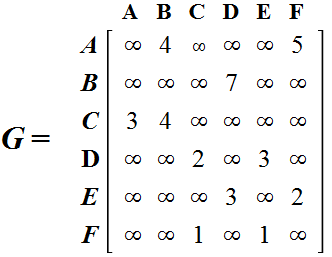
\includegraphics[width=0.5\textwidth]{Pictures/Teoriafsnit/Figurfiler/adjacency_matrix_weighted_directed_graph.PNG}
\end{adjustbox}
\caption{Nabo Matrix af orienteret vægtet graf}
\label{fig:adjacency-matrix-weighted-directed-graph}
\end{figure}

Grafteori er et vigtigt emne, da f.eks. korteste rute algoritmer som Dijkstra's har brug for at vide hvordan knuderne er forbundet, samt graden(hvor mange kanter knuden har) af den enktle knude, for at kun udregne den korteste rute. Derudover vil en grafmetode som en nabo-matix være en god måde at beskrive et vejnætværk på programerings niveau, da man kan have alle sine værdier i en variable.



\newpage
\section{Dijkstras Algoritme}
\begin{wrapfigure}{r}{0.45\textwidth}
    \centering
  \includegraphics[width=0.45\textwidth]{Pictures/Teoriafsnit/Figurfiler/DijkstraGraf.png}
  \label{dijkstrasgraf}
  \caption{En vægtet graf}
\end{wrapfigure}

Dijkstra's er en grådig algoritme der kan finde en rute imellem to knudepunkter i en vægtet graf. I gruppens program er dette eksempelvis ruten mellem et køretøjs hjem og destination. Algoritmen starter med at sætte afstanden til alle punkter lig uendelig, udover start punktet da det er det eneste der kendes til på tidspunktet. Når algoritmen kører en graf igennem, kigger den på den node hvor kosten er lavest, og udregner kosten til de naboliggende noder. Når kosten udregnes for en nabo node, tages kosten af ruten til den nuværende node og afstanden til nabo noden bliver adderet. Da algoritmen altid tager noden med den lavest kost, vil den have fundet den korteste rute, når den nuværende node er slutnoden \cite[s. 681-684]{DMATBOGEN}. Som et eksempel kan vejen fra A til Z på figur \ref{dijkstrasgraf} findes:

\begin{enumerate}
\item Algoritmen starter ved A, og kigger på naboerne B og C. Deres kost bliver noteret til at være 4 og 2.
\item Nu kigges der på noden C, da det er den nuværende korteste rute. Her ses det at kosten til B er 3 (2+1), og det bliver overskrevet da det er mindre end den tidligere værdi 4. Deruodver noteres det at kosten for D og E er 10 og 12.
\item Så kigges der på noden B, hvor det ses at kosten til D er 8 (2+1+5), og den overskriver den tidligere højere kost.
\item Derefter bliver noden D kigget på, hvor den noterer kosten for E og Z til at være 10 og 14. Selvom der er fundet en vej til slutnoden, forstættes der, da kosten til noden E er mindre end kosten til Z.
\item Så kigges der på noden E, hvor algoritmen ser at kosten til Z er 13, og dermed bliver den tidligere kost 14 overskrevet.
\item Der er ikke flere noder der har en lavere kost en slutnoden Z, og den korteste rute er fundet.
\end{enumerate}

Kostene for hver node kan gemmes i en tabel, som set på tabel \ref{dijktabel}.
  
\begin{table}[H]
\centering
  \begin{tabular}{|l|l|l|l|l|l|l|}
  \hline
                   & A & B & C & D  & E  & Z  \\ \hline
                   & 0 & $\infty$ & $\infty$ & $\infty$  & $\infty$  & $\infty$  \\ \hline
  A                & 0 & 4 & 2 & $\infty$  & $\infty$  & $\infty$  \\ \hline
  A, C             & 0 & 3 & 2 & 10 & 12 & $\infty$  \\ \hline
  A, C, B          & 0 & 3 & 2 & 8  & 12 & $\infty$  \\ \hline
  A, C, B, D       & 0 & 3 & 2 & 8  & 10 & 14 \\ \hline
  A, C, B, D, E    & 0 & 3 & 2 & 8  & 10 & 13 \\ \hline
  A, C, B, D, E, Z & 0 & 3 & 2 & 8  & 10 & 13 \\ \hline
  \end{tabular}
  \label{dijktabel}
  \caption{Dijkstra Kost Tabel}
\end{table}

\begin{figure}[H]
\begin{lstlisting}
object Node
  Previous = null
  Cost = PositiveInfinity

procedure FindPath(AllNodes, StartNode, EndNode)
  StartNode.Cost = 0
  List Closed.Add(AllNodes - StartNode)
    List Open.Add(StartNode)
    while Open > 0 do
      CurrentNode = Find Node with smallest Cost in Open
      if CurrentNode is EndNode
        return TracePath(CurrentNode)
      else
        Open.Remove(CurrentNode)
        Closed.Add(CurrentNode)
        EvaluateNeighbors(CurrentNode)
    end
    return null // No path found
end
\end{lstlisting}
\caption{Dijkstra pseudo-kode: FindPath og Node}\label{DijkstraCodeFindPathNode}
\end{figure}

På figur \ref{DijkstraCodeFindPathNode} ses pseudokode for kernen af Dijkstras algoritme. En \texttt{Node} er defineret først, hvor \texttt{Previous} til at starte med er \texttt{null} eller 'ikke eksisterende', og \texttt{Cost} er uendelig. \texttt{FindPath} proceduren tager en graph \texttt{AllNodes}, startnoden \texttt{StartNode} og slutnoden \texttt{EndNode}. Listerne \texttt{Open} og \texttt{Closed} bliver laver, og \texttt{Closed} fyldes med alle noderne bortset fra \texttt{StartNode}, da den skal findes i første iteration af while løkken. While løkken køres mens der stadig er noder der ikke er undersøgt, altså noder der ligger i \texttt{Open}, og den starter med at sætte \texttt{CurrentNode} til noden der har den laveste \texttt{Cost}. Hvis \texttt{CurrentNode} er lig \texttt{EndNode} så har algoritmen fundet ruten og den bliver returneret ved brug af proceduren \texttt{TracePath}, som beskrives sidst i dette afsnit. Hvis ikke \texttt{CurrentNode} er lig \texttt{EndNode}, så flyttes den til \texttt{Closed} listen og naboerne til noden bliver evalueret gennem proceduren \texttt{EvaluateNeighbors} som beskrives herunder.

\begin{figure}[H]
\begin{lstlisting}
procedure EvaluateNeighbors(CurrentNode)
  for each NeighborNode in CurrentNode
      if NeighborNode is not in Open
      and NeighborNode is not in Closed
        Open.Add(NeighborNode)
      NeighborNode.Cost = CurrentNode.Cost 
                        + DistanceTo(NeighborNode)
      if NeighborNode.Cost < CurrentNode.Cost
                             + DistanceTo(NeighborNode)
        NeighborNode.Previous = CurrentNode
  end
end
\end{lstlisting}
\caption{Dijkstra pseudo-kode: EvaluateNeighbors}\label{DijkstraCodeEvaluateNeighbors}
\end{figure}

\begin{figure}[H]
\begin{lstlisting}
procedure TracePath(CurrentNode)
  List Path
  while CurrentNode is not null
    Path.Add(CurrentNode)
    CurrentNode = CurrentNode.Previous
  end
  Path.Reverse()
  return Path
end
\end{lstlisting}
\caption{Dijkstra pseudo-kode: TracePath}\label{DijkstraCodeTracePath}
\end{figure}
\section{A* Algoritmen}\label{AStjerneTeori}
A* (A stjerne) er en udvidelse af Dijkstras algoritme. Forskellen ved A* algoritmen er at den estimerer hvor langt knuderne i graphen er fra slutknuden, og dermed findes den optimale rute hurtigere da den kun kigger på knuder der ligger i retningen af slutknuden. Dette gøres når nabo knuderne skal undersøges, ligesom i Dijkstra, vil algoritmen udregne kosten til nabo knuderne af det nuværende punkt, og derudover vil der benyttes en heuristik til at estimere kosten fra nabo knuden til slutknuden. Det vil sige at algoritmen arbejder med kosten til en knude, betegnet \texttt{G}, en heuristik der estimerer kosten fra knuden til slutknuden, betegnet \texttt{H}, og den samlede vurdering \texttt{F}, der udregnes som vist på formlen \ref{eq:A*}

\begin{equation} \label{eq:A*}
F(n) = G(n) + H(n)
\end{equation}
\vspace{5mm}

Hvis man ønsker at A* skal finde den absolut korteste rute, kræver det at heuristikken er optimistisk, altså at den aldrig overestimerer kosten til slutpunktet. Som et eksempel på en heuristik der kunne man definere heuristikken som værende afstanden i en lige linje til slutpunktet, da der aldrig ville være en kortere vej end dette. Yderligere, hvis man har informationen, kan der inddrages hastighedsgrænsen på vejene ved at dividere afstanden i en lige linje med den højste hastighedsgrænse der findes på vejnettet.

\vspace{5mm}

Estimationerne der bliver udregnet benyttes hver gang algoritmen skal vælge den næste \texttt{Node} der skal undersøges. Ligesom Dijkstra tager den knude der har den nuværende laveste \texttt{Cost}, tager A* den \texttt{Node} der har den laveste \texttt{Estimation} \texttt{F}.

\begin{figure}[H]
\begin{lstlisting}
object Node
  Previous = null
  Cost = PositiveInfinity
  Estimate = PositiveInfinity
  List NeighborNodes
\end{lstlisting}
\caption{A* pseudo-kode: Node}\label{AStarCodeNode}
\end{figure}

Forskellen på pseudokoden fra Dijkstras algoritme er lille. Til \texttt{Node} objektet, der ses på figur \ref{AStarCodeNode}, er der tilføjet \texttt{Estimate} variablen, der senere bliver udfyldt af \texttt{EvaluateNeighbors}.

\begin{figure}[H]
\begin{lstlisting}
CurrentNode = Node with smallest Estimate in Queue
\end{lstlisting}
\caption{A* pseudo-kode: Find smallest}\label{AStarCodeFindSmallest}
\end{figure}

I stedet for at sortere køen på \texttt{Cost} som der gøres i Dijkstra, bliver køen nu sorteret på \texttt{Estimate}, som set på figur \ref{AStarCodeFindSmallest}.

\begin{figure}[H]
\begin{lstlisting}
procedure EvaluateNeighbors(CurrentNode)
  for each NeighborNode in CurrentNode.NeighborNodes
    if NeighborNode is not in Queue
      Queue.Add(NeighborNode)
      PossibleCost = CurrentNode.Cost 
                     + distance from CurrentNode
                       to NeighborNode
      if NeighborNode.Cost > PossibleCost
        NeighborNode.Cost = PossibleCost
        NeighborNode.Previous = CurrentNode
        NeighborNode.Estimate = NeighborNode.Cost
                              + Heuristic(NeighborNode)
  end
end
\end{lstlisting}
\caption{A* pseudo-kode: EvaluateNeighbors}\label{AStarCodeEvaluateNeighbors}
\end{figure}

Den sidste ændring er fortaget i \texttt{EvaluateNeighbors}, set på figur \ref{AStarCodeEvaluateNeighbors}. Efter at en nabo \texttt{Node} er blevet fundet til at have en lavere \texttt{Cost} end den tidligere havde, bliver \texttt{Estimate} udregnet ved brug af knudens \texttt{Cost} eller \texttt{G}, plus heuristikken som eksempelvis kunne være distancen fra knuden til slutpunktet, som ses på linje 11 og 12 på figur \ref{AStarCodeEvaluateNeighbors}.















